\documentclass[mathserif,compress]{beamer} 

\usepackage{beamerthemeDresden} 
\usepackage[english]{babel}
\usepackage{amsmath,amssymb}
\usepackage[latin1]{inputenc}
\usepackage{palatino}
\usepackage{graphicx}
\usepackage{subfigure}
\usepackage{pgf}
\usepackage{relsize}
\beamertemplateshadingbackground{red!1}{blue!1}
% Use some nice templates
\beamertemplatetransparentcovereddynamic  
\usepackage{pgfpages} 

\def\beq{\begin{equation}}
\def\eeq{\end{equation}}
\def\bit{\begin{itemize}}
\def\eit{\end{itemize}}
\def\bdm{\begin{displaymath}}
\def\edm{\end{displaymath}}
\def\ben{\begin{enumerate}}
\def\een{\end{enumerate}}
\def\bc{\mathbf{c}}
\def\bh{\mathbf{h}}
\def\br{\mathbf{r}}
\def\bs{\mathbf{s}}
\def\bu{\mathbf{u}}
\def\bw{\mathbf{w}}
\def\bx{\mathbf{x}}
\def\by{\mathbf{y}}
\def\bz{\mathbf{z}}
\def\bA{\mathbf{A}}
\def\bD{\mathbf{D}}
\def\bG{\mathbf{G}}
\def\bI{\mathbf{I}}
\def\bQ{\mathbf{Q}}
\def\bR{\mathbf{R}}
\def\bS{\mathbf{S}}
\def\bV{\mathbf{V}}
\def\bW{\mathbf{W}}
\def\bX{\mathbf{X}}
\def\bY{\mathbf{Y}}
\def\bZ{\mathbf{Z}}
\def\cB{\mathcal{B}}
\def\cF{\mathcal{F}}
\def\cI{\mathcal{I}}
\def\cK{\mathcal{K}}
\def\cU{\mathcal{U}}
\def\bbeta{\mbox{\boldmath $\beta$}}
\def\bepsilon{\mbox{\boldmath $\epsilon$}}
\def\bdelta{\mbox{\boldmath $\delta$}}
\def\bgamma{\mbox{\boldmath $\gamma$}}
\def\bldeta{\mbox{\boldmath $\eta$}}
\def\bphi{\mbox{\boldmath $\phi$}}
\def\bkappa{\mbox{\boldmath $\kappa$}}
\def\blambda{\mbox{\boldmath $\lambda$}}
\def\bmu{\mbox{\boldmath $\mu$}}
\def\bnu{\mbox{\boldmath $\nu$}}
\def\btheta{\mbox{\boldmath $\theta$}}
\def\brho{\mbox{\boldmath $\rho$}}
\def\bDelta{\mbox{\boldmath $\Delta$}}
\def\bLambda{\mbox{\boldmath $\Lambda$}}
\def\bSigma{\mbox{\boldmath $\Sigma$}}
\def\var{\textrm{var}}
\def\cov{\textrm{cov}}
\def\log{\textrm{log}}
\def\median{\textrm{median}}
\def\argmin{\textrm{arg min }}
\def\bzero{\mathbf{0}}
\def\bone{\mathbf{1}}
\def\Poi{\textrm{Poi}}
\def\Unif{\textrm{Unif}}

%-------------------------------------------------------------------------------

\title[]{An Introduction to Statistical Models for Spatial Data in Ecology}

\author[Jay M. Ver Hoef]{Jay Ver Hoef} 

\institute[NOAA National Marine Mammal Lab]
{
	\normalsize NOAA National Marine Mammal Lab \\
	NOAA Fisheries \\
	International Arctic Research Center \\
	Fairbanks, Alaska, USA\\
	\vspace{0.1cm}
}
\date[04/15/13]{}
%-------------------------------------------------------------------------------
\begin{document}

%-------------------------------------------------------------------------------
\frame{\titlepage}
%-------------------------------------------------------------------------------

%-------------------------------------------------------------------------------
%                        OUTLINE
%-------------------------------------------------------------------------------

\section{Introduction}
\subsection{Outline}
\begin{frame} \frametitle{Outline}
     

	\begin{tabular} {p{3.8cm} p{5.8cm}}
	{
		\begin{center}
		\bit
			\item Introduction  \pause      
				\vspace{0.2cm}       
			\item Models  \pause         
				\vspace{0.2cm} 
			\item Inference  \pause    
				\vspace{0.2cm}      
			\item Simulations  \pause    
				\vspace{0.2cm}      
			\item Real Example \pause 
				\vspace{0.2cm}
			\item Summary
		\eit
	\end{center}
	} &
	{
		\vspace{.2cm}
%		\hspace{-.7cm}
		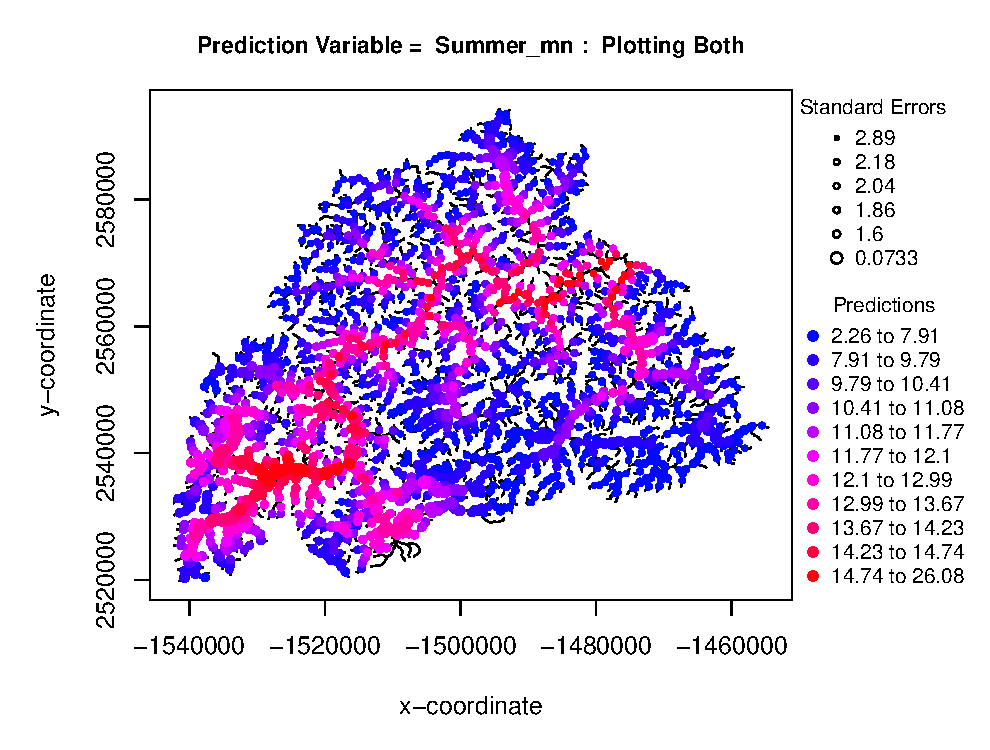
\includegraphics[width=5.8cm]{jss984Fig-Preds1} 
	}
	\end{tabular}

\end{frame}
   
%-------------------------------------------------------------------------------
%                        What Are Statistics?
%-------------------------------------------------------------------------------

\subsection{What are Statistics?}
\begin{frame} 
\frametitle{What are Statistics?}
     
	\begin{tabular} {p{5.8cm} p{3.8cm}}

			{\bdm
				\bar{z} = \frac{1}{n}\sum_{i = 1}^n z_i 
			\edm} &
			\vspace{.2cm}
			{A statistic is a function of data} 
		  \\
		
		\begin{center}
		  \vspace{-.5cm}
			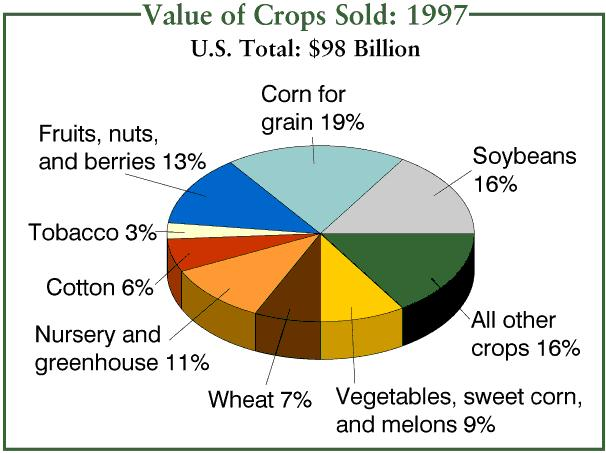
\includegraphics[width=3.0cm]{pieChart.jpeg} 
		  \vspace{.5cm}
		\end{center} &
		\begin{center}
		  \vspace{-.5cm}
			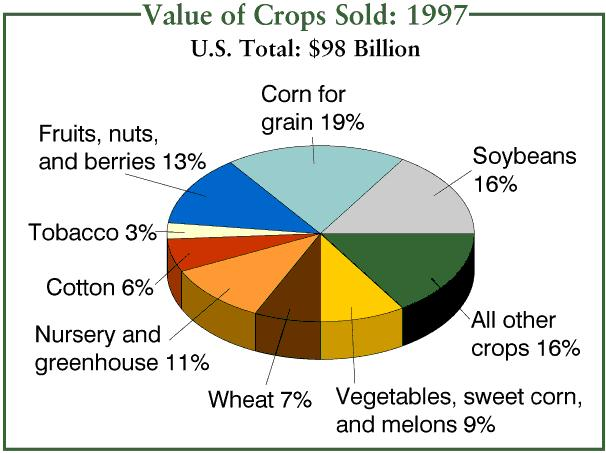
\includegraphics[width=3.0cm]{pieChart.jpeg} 
		  \vspace{.5cm}
		\end{center} 
		

	\end{tabular}

\end{frame}
 
%-------------------------------------------------------------------------------
%                        What Are Statistics?
%-------------------------------------------------------------------------------

\subsection{Statistical Models and Inference}
\begin{frame} 
\frametitle{Statistical Models and Inference}
     
		\begin{center}
		  \vspace{-.5cm}
			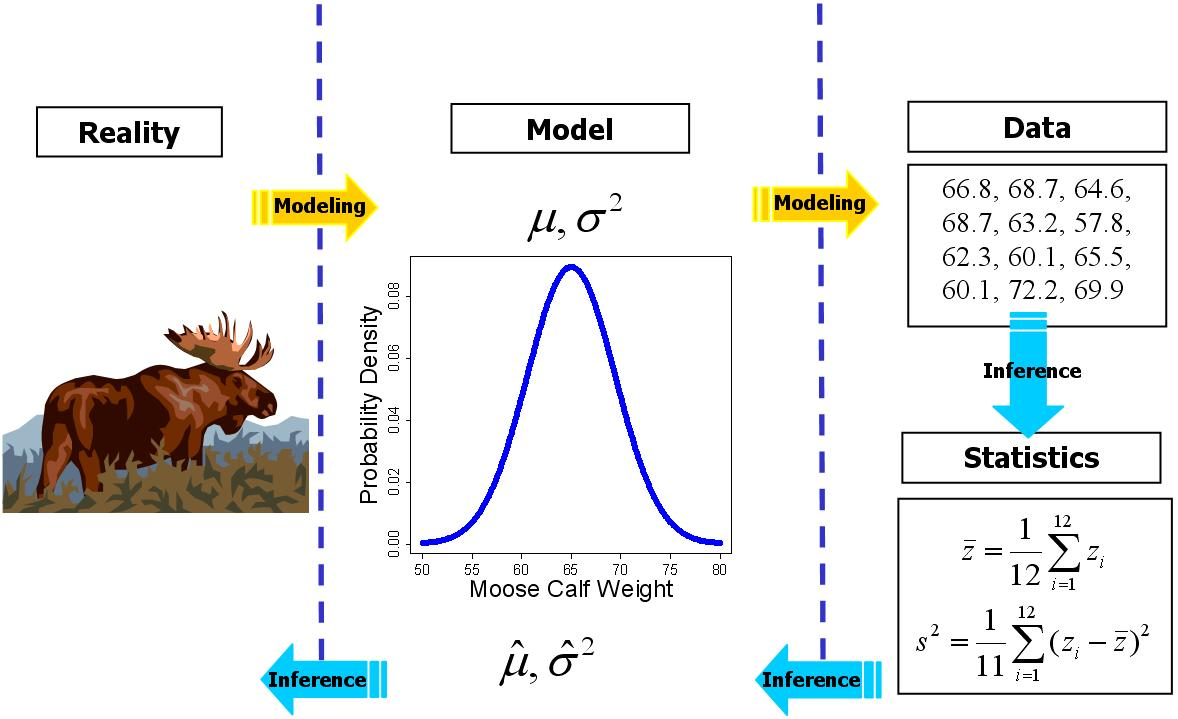
\includegraphics[width=10.4cm]{statModInfer.jpeg} 
		\end{center} 
\end{frame}


\end{document} 
